\section{Tabular Reinforcement Learning}

A trajectory $\tau$ is a sequence: $\tau \defeq (\tau_0, \tau_1, \tau_2, \dots)$, with $\tau_i \defeq (x_i, a_i, r_i, x_{i+1})$.
Agent can choose any policy $\rightarrow$ \textbf{on-policy} method. \\
No choice of policy $\rightarrow$ \textbf{off-policy} method. \\
\textbf{Model-based} $\rightarrow$ Learn the underlying MDP \\
\textbf{Model-free} $\rightarrow$ Learn value function directly.
All model-based methods are off-policy.
\begin{framed}
    \textbf{RM conditions}: $\alpha_t \geq 0$, $\sum_{t=0}^{\infty}{\alpha_t} = \infty$, $\sum_{t=0}^{\infty}{\alpha_t^2} < \infty$.
\end{framed}
\begin{framed}
    \textbf{Monte Carlo Control}
    Estimate underlying MDP using Monte carlo estimation:
    ${\hat{p}(x' \mid x, a) = \frac{N(x' \mid x, a)}{N(a \mid x)}}$ and \\ ${\hat{r}(x, a) = \frac{1}{N(a \mid x)} \sum_{t = 0, x_t = x,a_t = a}^\infty r_t}$
\end{framed}
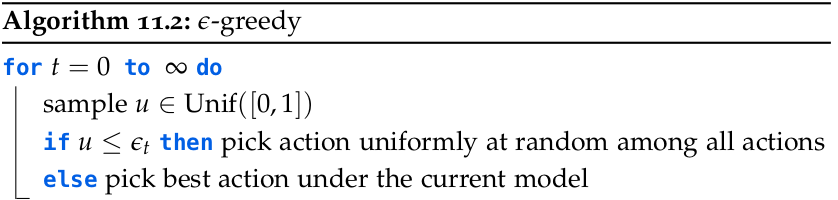
\includegraphics[width=0.95\linewidth,trim={0 0 3cm 0}]{images/epsilon_greedy.png}
\(\varepsilon\)-greedy converges to the optimal policy if the RM conditions are satisfied for \(\varepsilon_t\) and all state-action pairs are visited infinitely often.
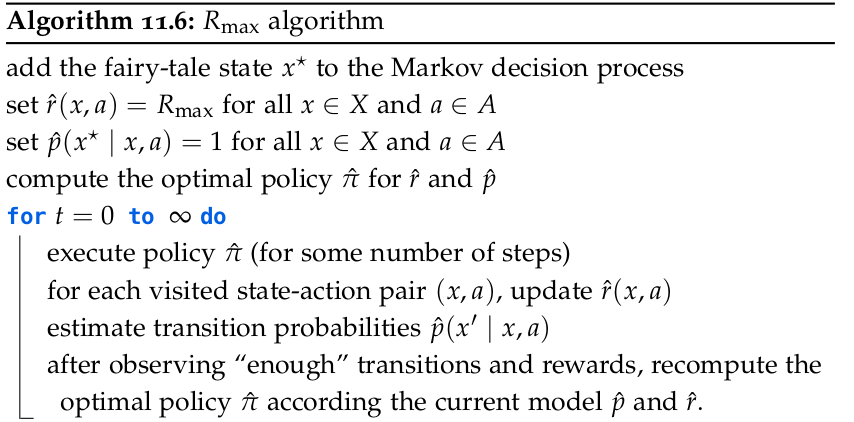
\includegraphics[width=0.95\linewidth, trim={0 0 3cm 0}]{images/R_max.png}
With probability at least $1-\delta$, $R_\mathrm{max}$ reaches an $\epsilon$-optimal policy in a number of steps that is polynomial in $\card{\sX}$, $\card{\sA}$, $T$, $\nicefrac{1}{\epsilon}$, $\nicefrac{1}{\delta}$, and $R_\mathrm{max}$.
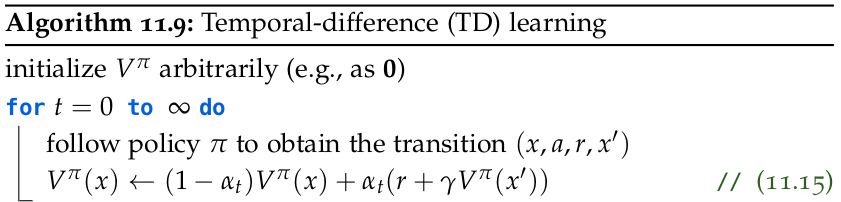
\includegraphics[width=0.95\linewidth,trim={0 0 4cm 0}]{images/TD_learning.png}
This is an on-policy method.
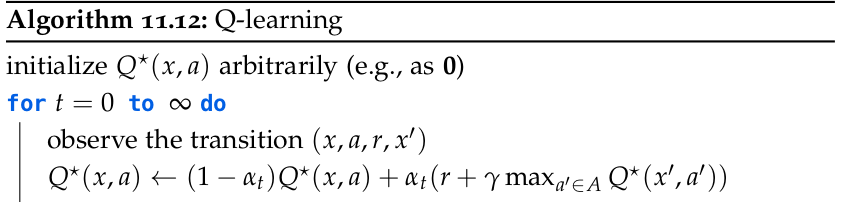
\includegraphics[width=0.95\linewidth, trim={0 0 3cm 0}]{images/Q_learning.png}
This is an off-policy method.
Optimistic: init $Q(x,a) = \frac{R_{\max}}{1-\gamma}$ for all $(x,a)$ pairs.
The update rule can also be expressed as: $\Q*{x}{a} \gets \Q*{x}{a} + \alpha_t\parentheses*{r + \gamma \max_{a' \in \sA} \Q*{x'}{a'} - \Q*{x}{a}}$.
Both converge if $\alpha_t$ satisfy RM conditions and every state-action pair is visited infinitely often.
RM: \(\alpha_t > 0, \sum_{t=1}^\infty \alpha_t = \infty, \sum_{t=1}^\infty \alpha_t^2 < \infty\). (Step sizes diminish but not too quickly.)

%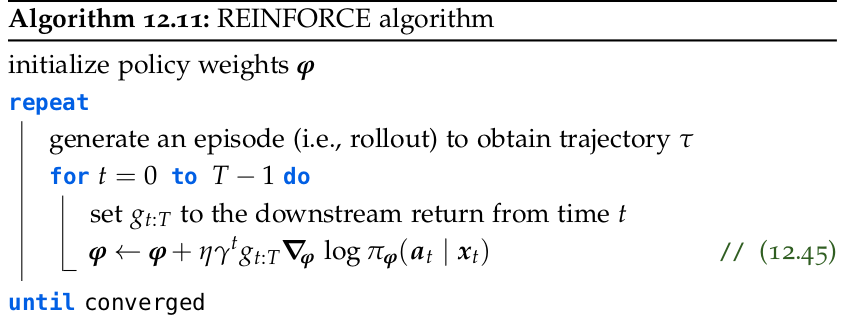
\includegraphics[width=\linewidth]{images/REINFORCE.png}
